% *********************************************************************
% © 2016–2024 Jeremy Sylvestre
%
% Permission is granted to copy, distribute and/or modify this document
% under the terms of the GNU Free Documentation License, Version 1.3 or
% any later version published by the Free Software Foundation; with no
% Invariant Sections, no Front-Cover Texts, and no Back-Cover Texts. A
% copy of the license is included in the appendix entitled “GNU Free
% Documentation License” that appears in the output document of this
% PreTeXt source code. All trademarks™ are the registered® marks of
% their respective owners.
%
% *********************************************************************
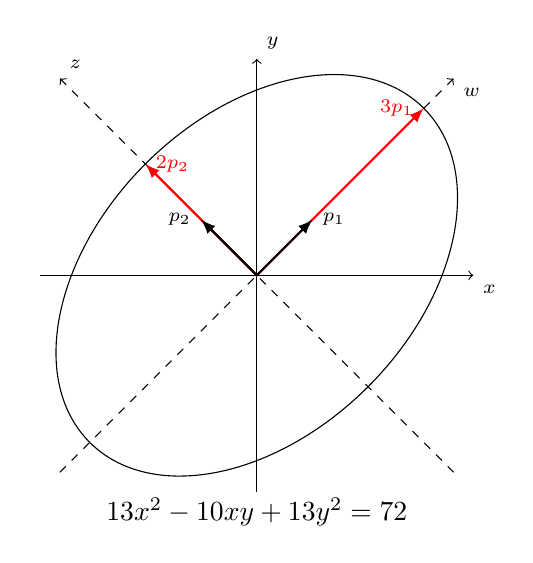
\begin{tikzpicture}[
	point/.style={circle,draw,very thin,fill,inner sep=0pt,minimum size=4pt},
	vector/.style={-latex},
]

	\draw[->] (-2.75,0) to (2.75,0) node[below right] {$\scriptstyle x$};
	\draw[->] (0,-2.75) to (0,2.75) node[above right] {$\scriptstyle y$};

	\draw[dashed,->] (2.5,-2.5) to (-2.5,2.5) node[above right] {$\scriptstyle z$};
	\draw[dashed,->] (-2.5,-2.5) to (2.5,2.5) node[below right] {$\scriptstyle w$};

	\draw[red,thick,vector] (0,0) to (2.121,2.121) node[left] {$\scriptstyle 3 \uvec{p}_1$};
	\draw[red,thick,vector] (0,0) to (-1.414,1.414) node[right] {$\scriptstyle 2 \uvec{p}_2$};

	\draw[thick,vector] (0,0) to (0.707,0.707) node[right] {$\scriptstyle \uvec{p}_1$};
	\draw[thick,vector] (0,0) to (-0.707,0.707) node[left] {$\scriptstyle \uvec{p}_2$};

	\draw[rotate=45] (0,0) ellipse (3cm and 2cm);

	\node at (0,-3) {$13 x^2 - 10 x y + 13 y^2 = 72$};

\end{tikzpicture}
